\section{Theorie}
\label{sec:Theorie}
Wasser kann die drei verschiedenen Zustände fest, flüssig und gasförmig annehmen. Mithilfe eine Zustandsdiagrammes lassen sich die 
Zustände qualitativ beschreiben (siehe \autoref{fig:zustandsdiagr}). In einem Zustandsdiagramm wird der Druck $p$ gegen die Temperatur $T$ 
aufgetragen und durch drei Kurven in drei verschiedene Teilbereiche eingeteilt. Die Grenzlinie zwischen fest und flüssig, die sogenannte 
Dampfdruckkurve hat eine viel geringere Steigung, als die fest-flüssig Kurve (Schmelzdruckkurve, siehe \cite{gerthsen}, S.301). Beide Kurven
treffen sich im \textit{Tripelpunkt} (T.P.). Im Tripelpunkt sind alle drei Phasen im Gleichgewicht koexistieren. Für Wasser liegt er bei 
$\SI{6.1}{\milli\bar}$ und $\SI{0.0075}{\celsius}$ (\cite{gerthsen}, S.301).
Innerhalb den drei Arealen hat das System zwei Freiheitsgrade $(T,p)$. 
Auf der Dampfdruckkurve jedoch, gibt es nur einen Freiheitsgrad.
%Ist eine feste Temperatur vorgegeben, so folgt auf einer der Kurven daraus ein fester Druck und andersherum.
Die Dampfdruckkurve wird im wesentlichen durch die molare Verdampfungswärme $L$ charakterisiert.

\begin{figure}[H]
    \centering
    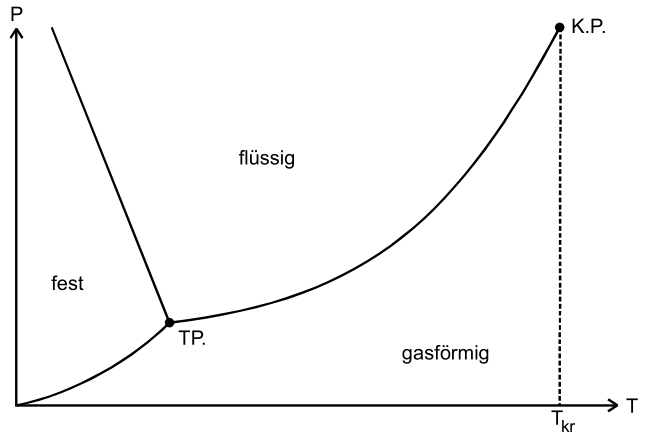
\includegraphics[width=0.75\textwidth]{daten/Zustandsdiagramm.png}
    \caption{Qualitatives Zustandsdiagramm \cite{anleitung}.}
    \label{fig:zustandsdiagr}
\end{figure}

\noindent
Wird eine Flüssigkeit in ein vollständig evakuiertes Gefäß gefüllt, so so verdampft ein Teil der Flüssigkeit in den Raum oberhalb der Flüssigkeit
selber. Es stellt sich nun ein charakteristischer Druck in diesem Raum, der \textit{Sättigungsdampfdruck}, ein.
Dieser Druck hängt nicht von dem Volumen des Gasraumes ab, da bei Änderung des Volumens ein Teil verdampft oder kondensiert, sodass das
Gleichgewicht wieder hergestellt ist.
Beim Prozess des Verdampfens verlassen diejenigen Moleküle die Flüssigkeitsoberfläche, die die dafür nötige kinetische Energie besitzen.
Sie leisten hierbei Arbeit gegen die Molekularkräfte, weshalb von außen Energie zum System hinzugeführt, oder dem Wärmevorrat entnommen werden
muss. Dies führt zur Abkühlung der Flüssigkeit. Die zur Umwandlung von einem Mol Wasser zu einem Mol Dampf bei gleicher Temperatur 
erforderliche Energie ist die zuvor genannte molare Verdampfungswärme $L \: [\si{\joule\per\mol}]$.
$L$ ist dabei eine stoff- und temperaturabhängige Größe, die im \textit{kritischen Punkt} (K.P.) fast vollständig verschwindet.


%Vielleicht umstrukturieren?

\noindent
Das System Dampf-Flüssigkeit lässt sich aufgrund des Gleichgewichtsdrucks nicht durch die allgemeine Gasgleichung 
\begin{align}
    \label{eqn:gasgl}
    pV = RT,
\end{align}
wobei $R$ die allgemeines Gaskonstante ist, beschreiben. Stattdessen wird einen Zusammenhang gewonnen, indem ein reversibler Kreisprozess
für ein Mol eines Stoffes durchgerechnet wird, der Volumen $V$ gegen Druck $p$ aufträgt. 
Eine qualitative Darstellung ist in \autoref{fig:kreisproz} abgebildet.

\begin{figure}[H]
    \centering
    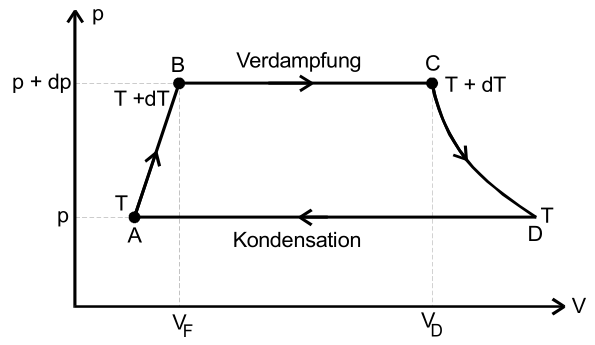
\includegraphics[width=0.75\textwidth]{daten/Dampfdruckkurve.png}
    \caption{Darstellung eines Kreisprozesses im pV-Diagramm \cite{anleitung}.}
    \label{fig:kreisproz}
\end{figure}

\noindent
Wird dem System eine Wärmemenge $\mathrm{d}{Q_{\text{AB}}}$ zugeführt. Dadurch steigt der Druck der Flüssigkeit auf 
$T+\mathrm{d}T$, der Druck auf $p+\mathrm{d}p$ 
und das Volumen auf  $V_{\text{F}}$ (Zustand B). Ein Teil der Flüssigkeit verdampft isotherm und isobar zu einem Gas mit Volumen 
$V_{\text{D}}$ (Zustand C). Ein Teil der Wärmeenergie wird wieder abgegeben auf $T$ und $p$ (Zustand D). Durch Kondensation wird
der Ausgangszustand A erreicht.
\\

\noindent
Die insgesamt bei dem Kreisprozess zugeführte Wärme erhält durch Summation dei einzelnen Wärmeenergien, unter Berücksichtigung des 
ersten Hauptsatzes der Thermodynamik den Ausdruck 
\begin{align}
    \label{eqn:gleichung1}
    (C_{\text{F}} - C_{\text{D}}) \mathrm{d}T + \mathrm{d}L = (V_{\text{D}} - V_{\text{F}}) \mathrm{d}p.
\end{align}

\noindent
Dabei entspricht $C_{\text{F}}$ der Molwärme der Flüssigkeit, $C_{\text{D}}$ der Molwärme des Dampfes und $\mathrm{d}L$ dem Unterschied 
der beiden Verdampfungswärmen. %$V_{\text{D}}, V_{\text{F}}$ entsprichen den beiden Volumina aus \autoref{fig:kreisproz}. 
Durch den zweiten Hauptsatz der Thermodynamik und unter der Vernachlässigung von Thermen 2.Ordnung folgt für (\ref{eqn:gleichung1})
\begin{align}
    (C_{\text{F}} - C_{\text{D}}) \mathrm{d}T + \mathrm{d}L - \frac{L\mathrm{d}T}{T}.
    \label{eqn:gleichung2}
\end{align}
Durch Vergleichen von (\ref{eqn:gleichung1}) und (\ref{eqn:gleichung2}) ergibt sich schließlich der Ausdruck
\begin{align}
    \label{eqn:CCDGL}
    (V_{\text{D}} - V_{\text{F}}) \mathrm{d}p = \frac{L}{T} \mathrm{d}T.
\end{align}
(\ref{eqn:CCDGL}) wird Clausius-Clapeyronsche Gleichung genannt. Wird eine Temperatur weit unter der kritischen Temperatur
$T_{\text{kritisch}}$ beschrieben, so können die Näherungen getroffen werden, dass $V_{\text{F}}$ gegenüber $V_{\text{D}}$ vernachlässigbar
ist und dass $V_{\text{D}}$ durch die ideale Gasgleichung (\ref{eqn:gasgl}) beschrieben werden kann. Außerdem sei $L$ druck- und
temperaturunabhängig. Dadurch folgt aus (\ref{eqn:CCDGL})
\begin{align*}
    \frac{R}{p}\mathrm{d}p=\frac{L}{T^2} \mathrm{d}T.
\end{align*}

\noindent
Woraus durch Integration folgt
\begin{align}
    \label{eqn:expo}
    p = p_0\cdot \exp(-\frac{L}{RT}).
\end{align}